\documentclass[conference]{IEEEtran}
\IEEEoverridecommandlockouts

\usepackage[utf8]{inputenc}
\usepackage[T1]{fontenc}
\usepackage{cite}
\usepackage{url}
\usepackage{array}
\usepackage{booktabs}
\usepackage{tabularx}
\usepackage{graphicx}
\usepackage{xcolor}
\usepackage{tikz}
\usetikzlibrary{arrows.meta, positioning, fit, shapes.geometric}

\definecolor{ttblue}{RGB}{37,99,160}
\definecolor{ttlight}{RGB}{232,241,250}
\definecolor{ttgray}{RGB}{245,245,245}
\definecolor{ttborder}{RGB}{90,90,90}

\title{TathyaTest: Generator Uji Fungsional, Regresi, dan Functional Availability Aplikasi Web}

\author{%
\IEEEauthorblockN{Nama Penulis Pertama\IEEEauthorrefmark{1}, Nama Penulis Kedua\IEEEauthorrefmark{2}}
\IEEEauthorblockA{\IEEEauthorrefmark{1}Program Studi ..., Institusi ..., Kota, Indonesia\\
Email: penulis1@example.ac.id}
\IEEEauthorblockA{\IEEEauthorrefmark{2}Program Studi ..., Institusi ..., Kota, Indonesia\\
Email: penulis2@example.ac.id}
}

\begin{document}

\maketitle

\begin{abstract}
TathyaTest menawarkan pipeline pembangkitan test case fungsional yang mengubah aplikasi web berjalan menjadi model elemen per role, matriks akses RBAC, dan spesifikasi Playwright yang dapat dieksekusi. Pendekatan ini dirancang untuk membantu tester membangun baseline pengujian regresi dan functional availability check tanpa menulis seluruh skrip end-to-end secara manual. Berbeda dari uptime monitoring yang hanya memeriksa apakah endpoint merespons, TathyaTest menargetkan fungsi yang dialami pengguna, seperti login, otorisasi berbasis peran, validasi formulir, CRUD, interaksi, dan pagination. Prototipe melakukan crawling terautentikasi menggunakan Playwright, mengekstraksi kontrak \texttt{crawl/<role>.json}, menghasilkan variasi data positif, negatif, dan edge, lalu mengemisi test suite Playwright untuk kategori auth, forms, interactions, pagination, dan RBAC. Makalah ini juga merumuskan kerangka evaluasi berbasis artefak QA, meliputi Crawl Success Rate, DOM Model Size, Generated Test Count, Scenario Coverage, Execution Outcome, Duplicate Test Title Count, dan Locator Fallback Rate. Dengan demikian, kontribusi makalah ini bukan klaim efektivitas defect detection yang luas, melainkan desain pipeline dan cara mengevaluasi potensi TathyaTest sebagai dasar pengujian regresi fungsional pada aplikasi web.
\end{abstract}

\begin{IEEEkeywords}
pengujian perangkat lunak, aplikasi web, test generation, regression testing, functional availability, Playwright, RBAC
\end{IEEEkeywords}

\section{Pendahuluan}

Aplikasi web modern membutuhkan pemeriksaan ketersediaan yang tidak berhenti pada status endpoint. Pada sistem akademik, layanan administrasi, e-commerce, dan aplikasi internal organisasi, pengguna menilai kualitas sistem dari keberhasilan login, akses halaman, pengisian formulir, dan perubahan data. Standar kualitas perangkat lunak menempatkan functional suitability, reliability, usability, security, dan maintainability sebagai karakteristik yang saling terkait, bukan sebagai dimensi yang berdiri sendiri \cite{iso25010}. Karena itu, uptime monitoring tetap penting sebagai bukti bahwa server merespons permintaan HTTP, tetapi bukti tersebut belum cukup untuk menilai apakah fungsi aplikasi tersedia bagi pengguna akhir.

Kesenjangan tersebut muncul karena technical availability dan functional availability menjawab pertanyaan yang berbeda. Sebuah aplikasi dapat mengembalikan status HTTP 200, tetapi login gagal karena perubahan konfigurasi session, formulir gagal dikirim karena perubahan validasi, pengguna biasa dapat mengakses halaman admin karena kesalahan otorisasi, atau tombol pagination tidak berfungsi karena perubahan DOM. Literatur pengujian fungsional menekankan bahwa test harus memeriksa perilaku eksternal dan oracle yang dapat diamati, bukan hanya status internal atau respons permukaan \cite{myers2011softwaretesting,ammann2016softwaretesting,iso29119}. Oleh sebab itu, functional availability perlu dibaca sebagai kemampuan menjalankan alur pengguna utama pada browser nyata.

Pengujian end-to-end (E2E) merupakan bukti yang relevan untuk functional availability karena test dijalankan melalui browser nyata. Penelitian web testing telah menunjukkan bahwa crawling UI, model halaman, fragmen web, dan screen transition dapat digunakan untuk membangun skenario test dari aplikasi yang berjalan \cite{ricca2001webanalysis,mesbah2012crawlajax,yandrapally2023fragment,le2025screen}. Namun, otomasi browser masih menuntut keputusan manual tentang skenario, locator, data uji, dan oracle, sementara test UI dikenal sensitif terhadap perubahan DOM, sinkronisasi asinkron, serta flakiness \cite{romano2021uiflaky,hashemi2022jsflaky,pei2023traf}. Bukti ini menunjukkan bahwa generator E2E perlu menghasilkan test yang dapat dieksekusi sekaligus artefak yang dapat diaudit kualitasnya.

Test-driven development (TDD) dan unit test tetap penting, tetapi keduanya tidak menggantikan pengujian perilaku eksternal. TDD membantu menjaga desain kode, aturan bisnis, dan unit logika internal; sementara itu, kegagalan integrasi antarmuka, perubahan struktur DOM, kegagalan login melalui browser, dan kesalahan akses antar peran sering muncul pada lapisan sistem. Studi tentang test automation maturity menunjukkan bahwa strategi otomasi, kualitas skrip, lingkungan test, dan integrasi CI berpengaruh terhadap nilai praktis otomasi, bukan sekadar jumlah test yang dibuat \cite{garousi2016automation,wang2022maturity,wang2022quality}. Dengan demikian, baseline E2E regression suite diperlukan sebagai pelengkap pengujian level kode, tetapi baseline tersebut harus memiliki locator, oracle, dan metrik maintainability yang dapat diperiksa.

Penelitian ini mengusulkan TathyaTest sebagai prototipe untuk menghasilkan baseline test suite dari aplikasi web yang sedang berjalan. TathyaTest membangun bukti melalui kontrak crawl per role, matriks akses RBAC, variasi data uji, dan spesifikasi Playwright yang dapat dieksekusi. Berbeda dari pendekatan yang bertumpu pada skrip rekaman atau deskripsi natural language, TathyaTest menekankan kontrak model elemen sebagai batas antara observasi browser dan pembangkitan test \cite{sunman2022automated,alian2024autoe2e,junior2025genia}. Dengan posisi tersebut, penelitian ini diarahkan untuk menjawab bagaimana pipeline dirancang, bagaimana akses berbasis role diturunkan dari crawl, dan bagaimana potensi prototipe dinilai tanpa mengklaim efektivitas empiris yang belum diuji.

Pertanyaan penelitian yang dibahas dalam makalah ini adalah sebagai berikut.

\begin{itemize}
    \item \textbf{RQ1:} Bagaimana merancang pipeline pembangkitan test case fungsional yang mengubah observasi DOM terautentikasi menjadi model elemen dan spesifikasi Playwright yang dapat dieksekusi?
    \item \textbf{RQ2:} Bagaimana crawl per role dapat digunakan untuk membentuk matriks akses dan menghasilkan kandidat test positif maupun negatif untuk skenario RBAC?
    \item \textbf{RQ3:} Artefak dan metrik QA apa yang paling tepat untuk menilai potensi TathyaTest sebagai baseline regresi dan functional availability check pada evaluasi awal?
\end{itemize}

Kontribusi makalah ini adalah sebagai berikut.

\begin{itemize}
    \item Mengusulkan arsitektur TathyaTest sebagai pipeline observasi DOM terautentikasi, pemodelan elemen, mapping intent, dan emisi Playwright untuk baseline regresi fungsional.
    \item Merumuskan kontrak \texttt{crawl/<role>.json} sebagai antarmuka auditabel antara crawler dan generator, sehingga test case diturunkan dari artefak observasi, bukan dari asumsi implisit generator.
    \item Merancang pembangkitan test yang mencakup auth, form, interaction, pagination, dan RBAC dengan spektrum positive, negative, dan edge berdasarkan constraint HTML serta konfigurasi data.
    \item Menyusun kerangka evaluasi berbasis artefak QA, termasuk Crawl Success Rate, Scenario Coverage, Execution Outcome, Duplicate Test Title Count, dan Locator Fallback Rate, sebagai dasar penilaian awal tanpa overclaim terhadap defect detection.
\end{itemize}

\section{Tinjauan Pustaka}

Automated test generation untuk aplikasi web menunjukkan bahwa skenario uji dapat dibangun dari artefak yang dapat diamati, bukan hanya dari skrip manual. Survei test generation dan search-based testing menunjukkan bahwa pembangkitan data dan test case telah lama menjadi tema utama dalam software testing \cite{mcminn2004searchbased,ali2010searchbased,anand2013orchestrated}. Pada domain web, studi sebelumnya memanfaatkan informasi penggunaan, model UI, crawling Ajax, atau fragmen halaman untuk menghasilkan skenario uji yang lebih sistematis \cite{ricca2001webanalysis,mesbah2012crawlajax,garcia2021webusage,yandrapally2023fragment}. Literatur ini mendukung asumsi bahwa observasi antarmuka dapat menjadi sumber test case, tetapi juga menunjukkan perlunya kontrak yang jelas antara hasil observasi dan test yang dieksekusi.

Dalam perspektif quality assurance, generator uji perlu dievaluasi sebagai bagian dari proses pengujian dinamis. ISO/IEC/IEEE 29119 mendefinisikan proses dan teknik pengujian, termasuk teknik berbasis spesifikasi yang relevan untuk menguji perilaku fungsional dari sudut pandang pengguna \cite{iso29119}. ISO/IEC 25010 menempatkan functional suitability, reliability, usability, security, maintainability, dan portability sebagai karakteristik kualitas produk perangkat lunak \cite{iso25010}. Selain itu, oracle problem menunjukkan bahwa test yang dihasilkan hanya bernilai bila memiliki mekanisme penilaian hasil yang dapat dipercaya \cite{barr2015oracle}; sementara mutation testing dan metamorphic testing menunjukkan bahwa kekuatan test suite tidak cukup dinilai dari jumlah test saja \cite{jia2011mutation,segura2016metamorphic}. Bukti tersebut mengarahkan evaluasi TathyaTest agar tidak hanya menghitung jumlah test case, tetapi juga menilai apakah test yang dihasilkan merepresentasikan fungsi penting, memiliki oracle yang dapat dieksekusi, dan mendukung regresi berulang.

Penelitian terkait regresi web juga menekankan keseimbangan antara otomasi dan maintainability. Studi regression testing menempatkan seleksi, minimisasi, prioritisasi, dan pemilihan ulang test sebagai isu utama ketika test suite berkembang \cite{rothermel2001prioritizing,elbaum2002prioritization,engstrom2010regression,yoo2012regression}. Pada aplikasi web, Yandrapally dan Mesbah \cite{yandrapally2023fragment} menunjukkan bahwa fragmen web dapat digunakan sebagai dasar pembangkitan uji, Garcia \emph{et al.} \cite{garcia2021webusage} memanfaatkan informasi penggunaan web, dan Abadeh \cite{abadeh2021webregression} mengusulkan framework evolusioner untuk auto-regression testing aplikasi web. Studi tentang page object dan web test maintenance menunjukkan bahwa abstraksi locator dapat membantu maintainability, tetapi pembuatan dan pemeliharaannya tetap menjadi pekerjaan signifikan \cite{leotta2016pageobject,stocco2018apogen,karagoz2026pageobject}. Karena itu, TathyaTest perlu menyertakan indikator seperti Duplicate Test Title Count dan Locator Fallback Rate agar kualitas artefak yang dihasilkan dapat ditelaah sebelum klaim efektivitas yang lebih luas dibuat.

RBAC membutuhkan strategi pengujian yang memisahkan perspektif pengguna. Model RBAC klasik menempatkan role sebagai perantara antara pengguna dan permission sehingga administrasi hak akses tidak melekat langsung pada individu \cite{ferraiolo1992rbac,sandhu1996rbac}. Literatur tentang autentikasi dan otorisasi juga menegaskan perbedaan antara verifikasi identitas dan keputusan akses, serta menempatkan RBAC sebagai salah satu model otorisasi yang umum digunakan \cite{margam2026auth}. Implikasinya, test generator perlu mengamati aplikasi dari beberapa role dan membandingkan permukaan akses yang ditemukan. Prinsip ini menjadi dasar crawling per role pada TathyaTest.

Makalah ini menempatkan kontribusi pada integrasi pipeline, bukan pada klaim bahwa satu teknik baru menyelesaikan seluruh masalah test generation. Bukti literatur menunjukkan adanya komponen yang relevan: observasi UI, pembangkitan uji, regresi, locator abstraction, flakiness, RBAC, dan E2E generation berbasis fitur \cite{mesbah2012invariant,sunman2022automated,romano2021uiflaky,hashemi2022jsflaky,pei2023traf,alian2024autoe2e,junior2025genia}. TathyaTest menggabungkan komponen tersebut melalui crawling per role, kontrak model elemen, pembangkitan variasi data, dan emisi spesifikasi Playwright. Dengan posisi ini, TathyaTest diperlakukan sebagai fondasi baseline regresi dan functional availability check yang masih memerlukan evaluasi empiris lanjutan.

\section{Metodologi Penelitian}

Penelitian ini menggunakan pendekatan rekayasa prototipe dengan orientasi design science karena tujuan utamanya adalah merancang dan menilai artefak perangkat lunak. Artefak yang dikaji adalah pipeline TathyaTest, mulai dari konfigurasi target, crawling terautentikasi, kontrak model elemen, mapping test case, sampai emisi Playwright. Pendekatan ini sesuai dengan tradisi penelitian software testing yang menilai artefak berdasarkan kemampuan menghasilkan test, oracle, dan bukti eksekusi \cite{bertolino2007testing,barr2015oracle,anand2013orchestrated}. Dengan demikian, evaluasi pada makalah ini dibatasi sebagai validasi tahap awal terhadap kelayakan desain.

Tahapan penelitian disusun agar setiap keputusan desain memiliki bukti artefaktual. Pertama, kebutuhan sistem dianalisis dari sudut pandang pengujian fungsional aplikasi web: login, peran pengguna, form CRUD, validasi, navigasi, search/filter, pagination, dan monitoring fungsional. Kedua, arsitektur dirancang dengan memisahkan lapisan crawling, kontrak model elemen, mapping test case, dan emitter Playwright. Ketiga, prototipe diimplementasikan sebagai CLI TypeScript yang memuat crawler Playwright, generator, dan runner test. Keempat, evaluasi awal dilakukan pada dua aplikasi Todo berbasis Laravel, yaitu versi Blade dan versi Inertia React, sehingga RQ3 dapat dijawab melalui artefak crawl, spesifikasi yang dihasilkan, dan hasil eksekusi test.

\section{Perancangan TathyaTest}

\subsection{Gambaran Umum Pipeline}

Pipeline TathyaTest dirancang agar setiap langkah menghasilkan artefak yang dapat diaudit. Seperti ditunjukkan pada Gambar~\ref{fig:tt-overview}, pengguna menyediakan aplikasi target, konfigurasi role, kredensial login, coverage, dan data uji; kemudian \texttt{tt crawl} menjalankan browser Playwright untuk setiap role, mengamati DOM setelah login, dan menulis kontrak JSON per role. Kontrak tersebut menjadi bukti observasi sebelum \texttt{tt generate} memetakannya menjadi intent test case dan spesifikasi Playwright. Alur ini menjawab RQ1 karena pembangkitan test tidak dilakukan langsung dari asumsi internal generator, tetapi dari model aplikasi yang diamati.

\begin{figure*}[!t]
\centering
\resizebox{0.98\textwidth}{!}{%
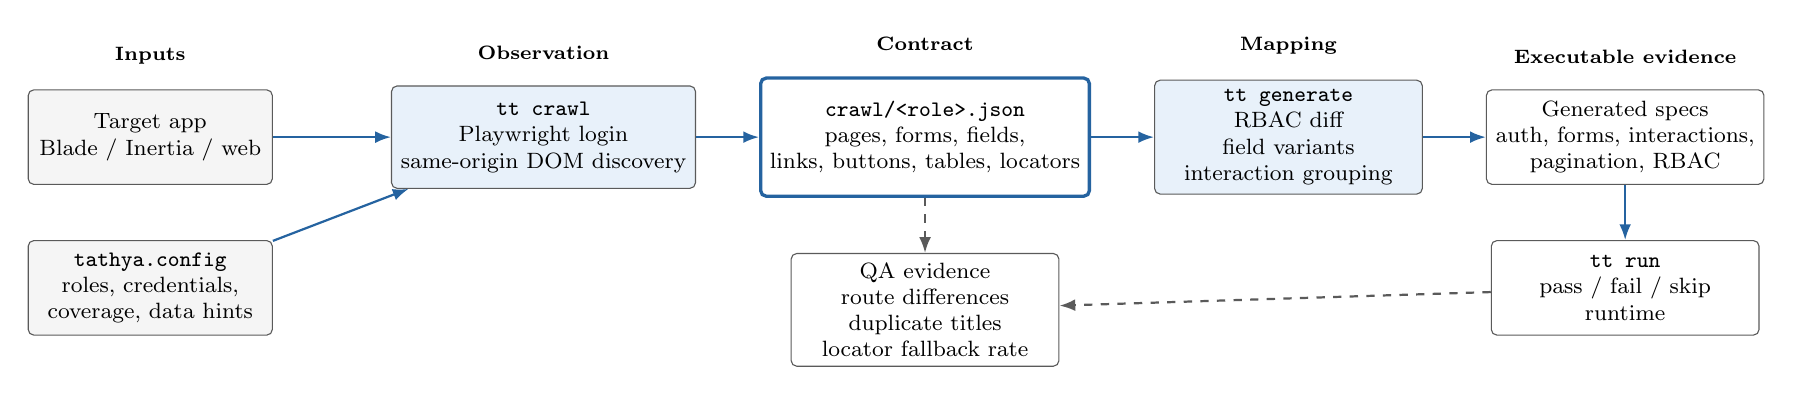
\begin{tikzpicture}[
    font=\footnotesize,
    node distance=7mm and 8mm,
    source/.style={draw=ttborder, rounded corners=2pt, fill=ttgray, align=center, minimum width=31mm, minimum height=12mm},
    process/.style={draw=ttborder, rounded corners=2pt, fill=ttlight, align=center, minimum width=34mm, minimum height=13mm},
    contract/.style={draw=ttblue, very thick, rounded corners=2pt, fill=white, align=center, minimum width=38mm, minimum height=15mm},
    evidence/.style={draw=ttborder, rounded corners=2pt, fill=white, align=center, minimum width=34mm, minimum height=12mm},
    label/.style={align=center, font=\scriptsize\bfseries},
    arrow/.style={-{Latex[length=2mm]}, thick, draw=ttblue},
    dashedarrow/.style={-{Latex[length=2mm]}, thick, dashed, draw=ttborder}
]
\node[source] (app) {Target app\\Blade / Inertia / web};
\node[source, below=of app] (config) {\texttt{tathya.config}\\roles, credentials,\\coverage, data hints};
\node[process, right=15mm of app] (crawl) {\texttt{tt crawl}\\Playwright login\\same-origin DOM discovery};
\node[contract, right=of crawl] (json) {\texttt{crawl/<role>.json}\\pages, forms, fields,\\links, buttons, tables, locators};
\node[process, right=of json] (map) {\texttt{tt generate}\\RBAC diff\\field variants\\interaction grouping};
\node[evidence, right=of map] (specs) {Generated specs\\auth, forms, interactions,\\pagination, RBAC};
\node[evidence, below=of specs] (run) {\texttt{tt run}\\pass / fail / skip\\runtime};
\node[evidence, below=of json] (qa) {QA evidence\\route differences\\duplicate titles\\locator fallback rate};
\node[label, above=2mm of app] {Inputs};
\node[label, above=2mm of crawl] {Observation};
\node[label, above=2mm of json] {Contract};
\node[label, above=2mm of map] {Mapping};
\node[label, above=2mm of specs] {Executable evidence};
\draw[arrow] (app) -- (crawl);
\draw[arrow] (config) -- (crawl);
\draw[arrow] (crawl) -- (json);
\draw[arrow] (json) -- (map);
\draw[arrow] (map) -- (specs);
\draw[arrow] (specs) -- (run);
\draw[dashedarrow] (json) -- (qa);
\draw[dashedarrow] (run) -- (qa);
\end{tikzpicture}}
\caption{Overview TathyaTest: dari konfigurasi dan aplikasi target menjadi kontrak crawl, spesifikasi Playwright, dan bukti QA yang dapat diaudit.}
\label{fig:tt-overview}
\end{figure*}

\subsection{Arsitektur Sistem}

Arsitektur TathyaTest memisahkan observasi aplikasi dan pembangkitan test agar pipeline dapat ditelaah secara bertahap. Lapisan CLI mengatur orkestrasi perintah, crawler Playwright melakukan login dan menemukan URL same-origin melalui DOM, generator memuat RBAC matrix builder, field variant generator, oracle generator, locator renderer, test case mapper, dan emitter, sedangkan execution layer menjalankan spesifikasi yang dihasilkan. Pemisahan tersebut dibuktikan oleh kontrak \texttt{crawl/<role>.json}: generator tidak membaca kode aplikasi target, tetapi hanya membaca model hasil observasi browser. Dengan demikian, kesalahan dapat dilacak apakah terjadi pada crawl, mapping, emisi spesifikasi, atau eksekusi test.

\subsection{Kontrak Model Elemen}

Kontrak model elemen menjadi bukti utama bahwa TathyaTest memisahkan hasil observasi dari logika pembangkitan test. Setiap role menghasilkan satu file JSON yang memuat daftar halaman, formulir, field, link, button, tabel, dan locator. Formulir menyimpan action, method, operasi CRUD, status \texttt{novalidate}, field, constraint, opsi, hint nama, serta locator submit. Struktur ini membuat generator dapat memproses aplikasi target secara deterministik dari model crawl, sehingga perubahan pada target app terlihat sebagai perubahan artefak sebelum menjadi perubahan test suite.

Locator dihitung dengan prioritas semantik untuk mengurangi risiko test yang rapuh. Urutannya adalah \texttt{data-testid}, role dan accessible name, label, placeholder, id stabil, atribut name, dan CSS fallback. Prioritas ini menyediakan bukti maintainability yang dapat dievaluasi melalui Locator Fallback Rate. Semakin kecil ketergantungan pada CSS fallback, semakin kuat indikasi bahwa test suite menggunakan selector yang dekat dengan cara pengguna atau tester mengenali elemen.

\subsection{Crawling Per Peran dan Matriks RBAC}

Untuk mendukung pengujian RBAC, TathyaTest menjadikan perbedaan hasil crawl antar role sebagai bukti akses. Sebuah rute dianggap reachable oleh role tertentu jika rute tersebut muncul pada hasil crawl role tersebut. Dengan membandingkan file crawl antar role, sistem membentuk access matrix; misalnya, rute yang muncul pada crawl admin tetapi tidak muncul pada crawl user menjadi kandidat test negatif untuk user. Mekanisme ini menjawab RQ2 karena kasus uji RBAC diturunkan dari observasi peran, bukan hanya dari daftar rute yang ditulis manual.

Pendekatan berbasis observasi mengurangi kebutuhan deklarasi eksplisit seluruh aturan RBAC, tetapi tidak menghapus keterbatasan crawler. Rute yang tidak muncul dalam DOM dan tidak dapat ditemukan melalui navigasi tidak akan masuk ke access matrix. Karena itu, konfigurasi \texttt{crawl.include} disediakan sebagai seed eksplisit untuk rute penting yang memang diketahui tester. Batasan ini penting agar hasil RBAC dipahami sebagai bukti dari permukaan aplikasi yang berhasil dicrawl.

\subsection{Pembangkitan Kasus Uji}

Mapper menjadi komponen yang mengubah bukti observasi menjadi intent pengujian. Kasus uji dibagi menjadi kelompok auth, form, interaction, pagination, dan RBAC. Untuk form, TathyaTest menghasilkan variasi data berdasarkan constraint field dan konfigurasi data: positive case menggunakan nilai valid, negative case mencakup pelanggaran validasi seperti field wajib kosong atau format salah, sedangkan edge case mencakup panjang batas, string panjang, Unicode, whitespace, dan penghilangan field opsional. Pembagian ini menjaga agar test yang dihasilkan tidak terbatas pada CRUD positif, tetapi mencakup spektrum positive, negative, dan edge sesuai kebutuhan QA.

Gambar~\ref{fig:generation-logic} memperjelas logika pembangkitan kasus uji. Crawler tidak langsung menghasilkan skrip Playwright, melainkan menghasilkan model antara. Generator kemudian membaca struktur halaman, formulir, link, button, tabel, dan locator; membandingkan rute antar role; membentuk variasi data; lalu menerjemahkan intent tersebut menjadi spesifikasi Playwright. Dengan demikian, nilai utama TathyaTest berada pada transformasi artefak observasi DOM menjadi test suite yang dapat diperiksa, bukan pada klaim bahwa semua kesalahan aplikasi otomatis ditemukan.

\begin{figure*}[!t]
\centering
\resizebox{0.98\textwidth}{!}{%
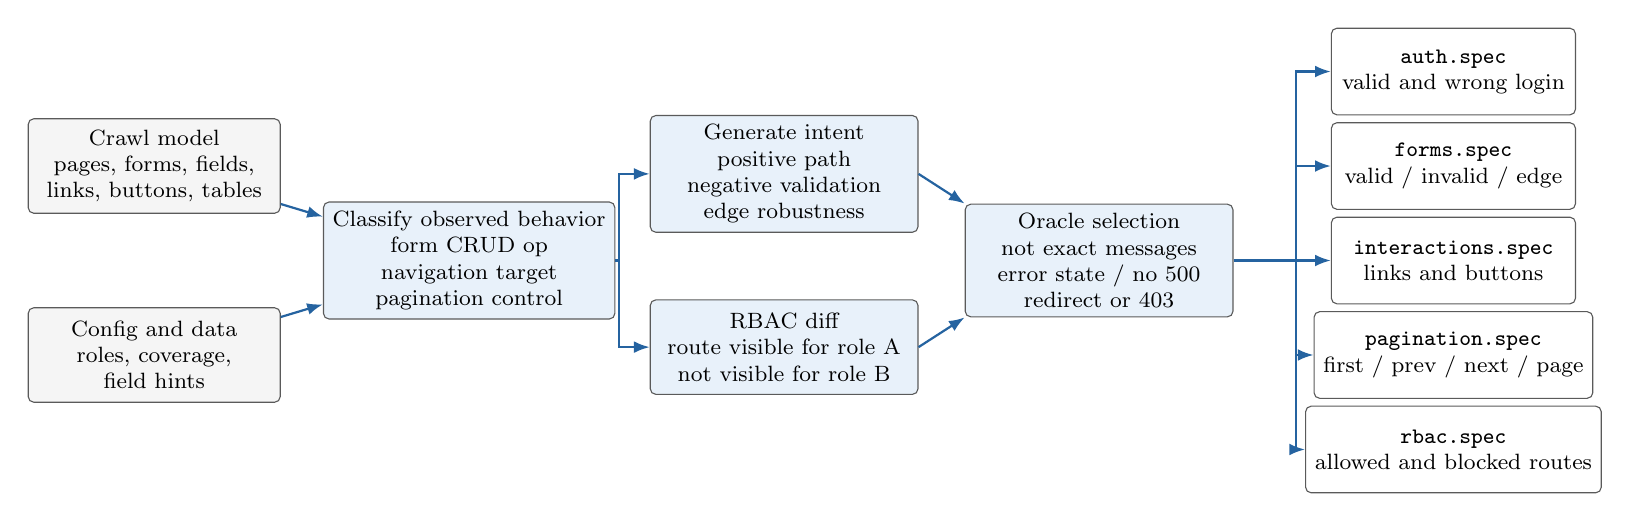
\begin{tikzpicture}[
    font=\footnotesize,
    x=1mm,
    y=1mm,
    source/.style={draw=ttborder, rounded corners=2pt, fill=ttgray, align=center, minimum width=32mm, minimum height=12mm},
    rule/.style={draw=ttborder, rounded corners=2pt, fill=ttlight, align=center, minimum width=34mm, minimum height=12mm},
    spec/.style={draw=ttborder, rounded corners=2pt, fill=white, align=center, minimum width=31mm, minimum height=11mm},
    arrow/.style={-{Latex[length=2mm]}, thick, draw=ttblue},
    bus/.style={thick, draw=ttblue}
]
\node[source] (pages) at (0,12) {Crawl model\\pages, forms, fields,\\links, buttons, tables};
\node[source] (config) at (0,-12) {Config and data\\roles, coverage,\\field hints};
\node[rule] (classify) at (40,0) {Classify observed behavior\\form CRUD op\\navigation target\\pagination control};
\node[rule] (variants) at (80,11) {Generate intent\\positive path\\negative validation\\edge robustness};
\node[rule] (rbac) at (80,-11) {RBAC diff\\route visible for role A\\not visible for role B};
\node[rule] (oracle) at (120,0) {Oracle selection\\not exact messages\\error state / no 500\\redirect or 403};
\node[spec] (auth) at (165,24) {\texttt{auth.spec}\\valid and wrong login};
\node[spec] (forms) at (165,12) {\texttt{forms.spec}\\valid / invalid / edge};
\node[spec] (interactions) at (165,0) {\texttt{interactions.spec}\\links and buttons};
\node[spec] (pagination) at (165,-12) {\texttt{pagination.spec}\\first / prev / next / page};
\node[spec] (rbacspec) at (165,-24) {\texttt{rbac.spec}\\allowed and blocked routes};
\coordinate (inputjoin) at (20,0);
\coordinate (intentjoin) at (59,0);
\coordinate (outbus) at (145,0);
\draw[arrow] (pages) -- (classify);
\draw[arrow] (config) -- (classify);
\draw[bus] (classify.east) -- (intentjoin);
\draw[arrow] (intentjoin) |- (variants.west);
\draw[arrow] (intentjoin) |- (rbac.west);
\draw[arrow] (variants.east) -- (oracle.north west);
\draw[arrow] (rbac.east) -- (oracle.south west);
\draw[bus] (oracle.east) -- (outbus);
\draw[arrow] (outbus) |- (auth.west);
\draw[arrow] (outbus) |- (forms.west);
\draw[arrow] (outbus) -- (interactions.west);
\draw[arrow] (outbus) |- (pagination.west);
\draw[arrow] (outbus) |- (rbacspec.west);
\end{tikzpicture}}
\caption{Logic flow pembangkitan test case: observasi DOM dan konfigurasi diubah menjadi intent, oracle, lalu file spesifikasi Playwright.}
\label{fig:generation-logic}
\end{figure*}

Oracle assertion dirancang untuk memeriksa state, bukan teks pesan yang rapuh. Untuk form dengan \texttt{novalidate}, sistem mengecek indikator error pada DOM dan memastikan halaman kembali ke konteks form. Untuk validasi native HTML5, sistem mengecek validity state atau selector \texttt{:invalid}. Bukti ini penting karena error message sering berubah antar bahasa, framework, dan desain UI; dengan demikian, oracle berbasis state lebih sesuai untuk baseline regresi yang perlu bertahan terhadap perubahan presentasi.

\subsection{Functional Availability}

TathyaTest memperluas availability ke arah fungsi yang dialami pengguna. Uptime monitoring tradisional memberi bukti bahwa server dapat dijangkau melalui HTTP 200, ping, atau response time. Functional availability check memberi bukti tambahan bahwa alur penting seperti login, akses role, CRUD, validasi form, search/filter, pagination, dan aksi perubahan data masih dapat dijalankan. Dengan framing ini, TathyaTest tidak menggantikan monitoring infrastruktur, tetapi menyediakan kandidat synthetic check yang lebih dekat dengan pengalaman pengguna.

\section{Implementasi Prototipe}

Prototipe TathyaTest diimplementasikan sebagai komponen TypeScript terpadu agar crawling dan emisi test berada pada satu toolchain. Di dalamnya terdapat crawler Playwright untuk autentikasi per role, crawling same-origin dari DOM, validasi konfigurasi, RBAC diff, field variant generator, oracle, mapper, dan emitter Playwright. Keputusan menggunakan satu engine memberi bukti perilaku browser yang konsisten untuk target server-rendered dan JavaScript-rendered. Hal ini mendukung tujuan penelitian karena evaluasi tidak bergantung pada perbedaan crawler statis dan crawler browser.

CLI \texttt{tt} menyediakan bukti operasional bahwa pipeline dapat dijalankan sebagai alur QA berulang. Perintah \texttt{tt init} membuat konfigurasi awal, \texttt{tt crawl} menjalankan crawler Playwright, \texttt{tt generate} membaca hasil crawl dan menghasilkan spesifikasi Playwright, \texttt{tt run} menjalankan test suite, dan \texttt{tt all} menjalankan seluruh pipeline dari crawl sampai eksekusi. Struktur perintah ini menghubungkan desain pada RQ1 dengan praktik penggunaan oleh tester.

Dua aplikasi studi kasus disediakan untuk memberi variasi mekanisme rendering pada domain yang sama. Aplikasi pertama adalah Laravel Breeze Blade Todo App yang merepresentasikan aplikasi server-rendered, sedangkan aplikasi kedua adalah Laravel Breeze Inertia React Todo App yang merepresentasikan aplikasi JavaScript-rendered. Keduanya memiliki fitur login, admin/user role, Todo CRUD, done/undone, search, filter, pagination, validasi form, dan halaman admin-only. Kesamaan fitur tersebut membuat perbedaan hasil lebih mudah ditelusuri ke mekanisme rendering atau pipeline TathyaTest, bukan ke perbedaan domain aplikasi.

\section{Evaluasi Tahap Awal}

\subsection{Tujuan Evaluasi}

Evaluasi tahap awal bertujuan menjawab RQ3 dengan menilai apakah artefak TathyaTest cukup untuk menjadi baseline test suite. Bukti yang diamati adalah keberhasilan crawl terautentikasi, kelengkapan model elemen, keunikan test case, kemampuan eksekusi Playwright, dan representasi skenario fungsional penting. Bukti tersebut relevan untuk QA karena menunjukkan apakah pipeline menghasilkan sinyal yang dapat dipakai tester. Namun, evaluasi ini tidak dimaksudkan untuk membuktikan fault detection superiority atau efektivitas statistik pada banyak aplikasi.

\subsection{Objek Evaluasi}

Objek evaluasi dipilih untuk memeriksa pipeline pada dua mekanisme rendering yang umum. Aplikasi Blade merepresentasikan server-rendered web app, sedangkan aplikasi Inertia React merepresentasikan JavaScript-rendered web app. Keduanya dicrawl menggunakan engine Playwright yang sama dan dibuat dengan fitur paralel. Dengan desain ini, bukti evaluasi dapat dibandingkan pada fungsi yang serupa tanpa menjadikan perbedaan domain sebagai faktor utama.

\subsection{Alur Evaluasi}

Alur evaluasi dibuat berulang agar setiap hasil dapat ditelusuri ke artefak yang jelas. Urutannya adalah menyiapkan basis data, menjalankan \texttt{tt crawl}, menjalankan \texttt{tt generate}, menjalankan Playwright, lalu menghitung metrik dari artefak yang dihasilkan. Urutan ini memisahkan tiga sumber kegagalan: aplikasi target yang tidak berjalan benar, crawler yang gagal membentuk model, dan generator yang menghasilkan suite tidak valid. Pemisahan tersebut memperkuat interpretasi RQ3 karena kegagalan tidak langsung disimpulkan sebagai kelemahan seluruh pipeline.

\subsection{Skenario Evaluasi}

Skenario evaluasi harus mencerminkan fungsi yang secara langsung dialami pengguna. Tabel~\ref{tab:scenarios} merangkum skenario login, RBAC, CRUD, validasi, search/filter, pagination, dan aksi perubahan state. Skenario tersebut menjadi bukti target fungsional yang diharapkan muncul dalam test suite. Jika suatu skenario tidak direpresentasikan oleh hasil generate, gap tersebut dapat ditelusuri pada crawl model atau aturan mapping.

\begin{table}[!t]
\caption{Skenario Evaluasi Tahap Awal}
\label{tab:scenarios}
\centering
\begin{tabularx}{\linewidth}{p{0.12\linewidth}X X}
\toprule
ID & Skenario & Tujuan \\
\midrule
S1 & Login admin dan user & Memvalidasi alur autentikasi \\
S2 & Admin membuka halaman admin & Positive RBAC \\
S3 & User membuka halaman admin & Negative RBAC \\
S4 & Create dan update todo & Positive CRUD \\
S5 & Submit form invalid & Negative validation \\
S6 & Input panjang, Unicode, whitespace & Edge behavior \\
S7 & Search dan filter todo & Interaksi form GET \\
S8 & Pagination todo & Navigasi data \\
S9 & Toggle done/undone & Aksi perubahan state \\
S10 & Delete todo & Aksi destruktif \\
\bottomrule
\end{tabularx}
\end{table}

\subsection{Metrik Evaluasi Awal}

Metrik evaluasi dipilih untuk menilai rantai artefak, bukan hanya volume test. Tabel~\ref{tab:metrics} merangkum metrik yang dikumpulkan dari \texttt{crawl/<role>.json}, file \texttt{tests/generated}, dan keluaran Playwright. Crawl Success Rate dan DOM Model Size memberi bukti observasi aplikasi, Generated Test Count dan Scenario Coverage memberi bukti mapping, sedangkan Execution Outcome memberi bukti eksekusi. Nama metrik dipertahankan dalam bahasa Inggris agar konsisten dengan istilah QA dan tidak disalahartikan sebagai placeholder hasil.

\begin{table}[!t]
\caption{Functional QA Metrics for TathyaTest}
\label{tab:metrics}
\centering
\begin{tabularx}{\linewidth}{p{0.29\linewidth}X}
\toprule
Metric & Operational meaning \\
\midrule
Crawl Success Rate & proportion of configured roles that produce valid crawl files \\
DOM Model Size & number of pages, forms, fields, links, buttons, tables, and locators extracted \\
Generated Test Count & number of unique tests emitted per spec category \\
Scenario Coverage & S1--S10 functional scenarios represented by at least one generated test \\
Execution Outcome & pass, fail, skip, and runtime from Playwright execution \\
RBAC Route Difference & routes visible to one role but absent or blocked for another role \\
Duplicate Test Title Count & duplicate Playwright test titles in generated specs \\
Locator Fallback Rate & proportion of locators that fall back to CSS rather than semantic selectors \\
\bottomrule
\end{tabularx}
\end{table}

Metrik maintainability diperlukan karena test yang banyak belum tentu bernilai bagi tester. Evaluasi juga mencatat waktu \texttt{tt crawl}, waktu \texttt{tt generate}, jumlah file spesifikasi, dan jumlah test yang di-skip. Skip rate dihitung sebagai jumlah test skip dibagi total test yang dijalankan, sedangkan Locator Fallback Rate dihitung sebagai jumlah locator CSS dibagi total locator. Kedua metrik ini tidak membuktikan kebenaran aplikasi, tetapi membantu menilai apakah suite yang dihasilkan representatif dan layak dipelihara.

\begin{table}[!t]
\caption{Evidence Matrix and Interpretation}
\label{tab:evidence}
\centering
\begin{tabularx}{\linewidth}{p{0.30\linewidth}XX}
\toprule
Evidence & Source & Interpretation \\
\midrule
Crawl model & \texttt{crawl/*.json} & observed functional surface per role \\
Generated specs & spec files & executable test intent, grouped by concern \\
Playwright outcome & test report & whether generated suite gives an execution signal \\
RBAC difference & per-role route diff & candidate positive and negative authorization cases \\
Duplicate title count & generated spec scan & suite validity before execution \\
Locator distribution & crawl locators & maintainability risk indicator \\
\bottomrule
\end{tabularx}
\end{table}

\subsection{Interpretasi Bukti Evaluasi}

Interpretasi evaluasi harus mengikuti bukti yang benar-benar dihasilkan oleh pipeline. Naskah ini tidak menggunakan tabel placeholder sebagai bukti hasil; nilai numerik harus diperoleh dari eksekusi ulang pipeline pada masing-masing studi kasus: penyiapan basis data, \texttt{tt crawl}, \texttt{tt generate}, dan Playwright test run. Setelah nilai tersebut tersedia, Crawl Success Rate dapat digunakan untuk membaca keberhasilan autentikasi dan observasi DOM, Scenario Coverage untuk membaca representasi fungsi, Execution Outcome untuk membaca sinyal eksekusi, Duplicate Test Title Count untuk membaca validitas suite Playwright, dan Locator Fallback Rate untuk membaca risiko maintainability. Dengan batasan ini, evaluasi tetap berguna tanpa membuat klaim yang melampaui data.

Dengan kerangka ini, potensi TathyaTest tidak disimpulkan dari jumlah test semata. Potensi dinilai dari rantai bukti: fungsi ditemukan oleh crawler, direpresentasikan dalam kontrak model, dipetakan menjadi test unik, dieksekusi oleh Playwright, dan menghasilkan sinyal yang dapat dipakai tester untuk regresi atau functional availability check. Klaim yang lebih kuat, seperti fault detection rate, flaky test rate, atau penurunan biaya manual testing, memerlukan eksperimen tambahan dan tidak diklaim dalam evaluasi awal ini.

\section{Diskusi}

Nilai utama TathyaTest berada pada penyusunan baseline QA dari aplikasi yang sedang berjalan. Metrik pada Tabel~\ref{tab:metrics} menyediakan bukti untuk menilai tiga potensi tersebut: pengurangan pekerjaan awal pembuatan E2E regression suite, pembentukan RBAC-aware testing melalui crawl per role, dan penggunaan suite sebagai kandidat functional availability check. Ketiga potensi ini hanya kuat jika model DOM cukup lengkap, locator cukup stabil, test yang dihasilkan unik, dan hasil eksekusi memberi sinyal yang dapat ditindaklanjuti. Karena itu, diskusi TathyaTest harus dibaca sebagai analisis potensi berbasis artefak, bukan klaim efektivitas umum.

Keterbatasan utama TathyaTest berasal dari sumber bukti yang digunakan, yaitu DOM dan konfigurasi. Crawler hanya dapat mengekstraksi informasi yang tampak pada DOM atau dapat diturunkan dari atribut HTML, sehingga aturan validasi server yang kompleks, seperti closure validation atau aturan bisnis khusus, tidak selalu dapat diekstraksi otomatis. Kualitas locator juga bergantung pada kualitas markup aplikasi target; aplikasi tanpa label, accessible name, atau atribut stabil dapat menghasilkan locator yang lebih rapuh. Selain itu, evaluasi tahap awal masih terbatas pada dua studi kasus Laravel dan belum mencakup aplikasi produksi skala besar, mutation score, fault detection rate, flaky test rate, atau maintenance cost.

Keterbatasan tersebut menentukan cara membaca kontribusi makalah. Bukti yang tersedia cukup untuk menjelaskan desain pipeline dan kerangka evaluasi awal, tetapi belum cukup untuk menyimpulkan superioritas terhadap penulisan test manual atau tool lain. Oleh karena itu, makalah ini menempatkan TathyaTest sebagai prototipe dan fondasi penelitian lanjutan, bukan sebagai solusi final yang telah divalidasi pada semua konteks aplikasi web.

\section{Kesimpulan dan Pekerjaan Lanjutan}

Makalah ini menyajikan TathyaTest sebagai rancangan generator kasus uji fungsional berbasis crawling untuk aplikasi web. Bukti desainnya adalah pipeline yang melakukan crawling per role, mengekstraksi model elemen ternormalisasi, membentuk matriks RBAC, menghasilkan variasi data uji, dan mengemisi spesifikasi Playwright. Kerangka evaluasi yang diusulkan menilai artefak tersebut melalui model crawl, jumlah test unik, cakupan skenario, hasil eksekusi, dan indikator maintainability. Dengan demikian, kontribusi utama makalah ini adalah desain pipeline dan kerangka evaluasi awal untuk baseline regresi dan functional availability, bukan klaim efektivitas empiris yang luas.

Pekerjaan lanjutan perlu memperkuat bukti empiris yang belum tersedia pada evaluasi awal. Evaluasi kuantitatif pada lebih banyak aplikasi, pengukuran coverage, fault detection rate, flaky test rate, waktu generasi, dan perbandingan dengan penulisan test manual diperlukan untuk menilai dampak praktis TathyaTest. Selain itu, penelitian lanjutan perlu memperluas dukungan terhadap aturan validasi server-side yang kompleks, meningkatkan robust locator generation, dan mengevaluasi integrasi TathyaTest dalam pipeline CI/CD untuk synthetic functional monitoring setelah deployment. Arah ini menghubungkan kontribusi prototipe dengan kebutuhan validasi akademik dan praktik QA yang lebih kuat.

\section*{Ucapan Terima Kasih}

Bagian ini dapat diisi dengan sumber pendanaan, dukungan institusi, atau pihak yang membantu pengembangan studi kasus dan evaluasi.

\bibliographystyle{IEEEtran}
\bibliography{tathyatest-references}

\end{document}
